\section{计算机制与情景检验细节}\label{app:science}
本附录保留容量约束、收支切换、参数敏感性及经济情景的计算细节。正文的财务与社会收益比较复用这些计算入口；具体演示值用于检查公式和展示方案变化。
\subsection{操作自测口径与原始计时}

2026年10月15日，在服务已启动、两份求是村原文已归档并完成解析的条件下，固定两个问题及五项核对标准：供水楼幢、252户范围、留博楼排除原因、报道时点的进场阶段、加梯征求意见阶段。Codex分别执行逐份查看与工作台检索两条自动浏览器路径，五项均可回到原文核对。计时从路径操作开始至读取对应内容结束，资料获取、导入及人工被试时间不在计时范围。

逐份查看路径耗时8.851秒；工作台路径耗时39.389秒，包含一次对未登记举措筛选条件的纠正。另行测得两次本地检索接口响应为29.777与19.498毫秒，合计49.275毫秒，前五条结果找回三处预先登记的目标片段（3/3）。自动操作耗时与接口响应分别记录；本次为单项目操作自测，未开展人工被试实验，不由接口毫秒数或两条自动路径推算人工节时率。完整问题、范围、返回定位、计时及操作条件见\path{research/test_results/decision-value-selftest-20261015.json}。

\subsection{用分时容量纠正月度合计的乐观假设}

服务需求具有时段差异，月平均量会掩盖高峰时段的供给不足。\cite{green2007} 在预约无法改期、服务不能跨时段结转的假设下，设第$t$时段需求为$D_t$、有效容量为$K_t$，则
\begin{equation}
 V=\sum_t\min(D_t,K_t),\qquad
 U=\frac{V}{\sum_tK_t},\qquad
 L=\sum_t\max(0,D_t-K_t).
\end{equation}
这里$V$为服务人次，$U$为容量利用率，$L$为未满足需求人次。由于
\begin{equation}
 \sum_t\min(D_t,K_t)\leq\min\!\left(\sum_tD_t,\sum_tK_t\right),
\end{equation}
月合计计算应被理解为需求可在容量间匹配时的上限。演示中两时段需求为80、20人次，容量各为50人次；分时结果为70人次、未满足30人次、利用率70\%，月合计上限则为100人次。系统同时显示两种结果及30人次的高估量。

界面已支持逐时段输入需求、场次、每场容量及其依据；启用后按分时记录计算。一个时段类别内部仍需说明需求能够匹配该类场次。当前保留独立资源检查，共用场地需要先明确分配；研究并未引入未经校准的随机排队或预约改期模型。

\subsection{用收支切换值说明结论离边界有多远}

Green Book将敏感性分析与切换值用于识别改变方案判断的关键条件。\cite{greenbook2026} 月度运营核算先区分运营方现金与财政支付。设服务人次为$V$、收费比例为$q$、每收费人次价格为$p$、每人次变动成本为$v$、固定运营支出为$F$，其他经营收入为$R_o$、政府购买服务为$G_p$、运营补贴为$S$、其他支持为$H$，则
\begin{equation}
 \Pi=V(qp-v)+R_o+G_p+S+H-F.
\end{equation}
政府直接支付的其他运营费用另列，不重复进入运营方支出；财政支出按政府购买服务、补贴和政府直接支付汇总。建设投资、贷款本息和折旧沿用建设经济模型。

对单一服务，保持价格、收费比例、单位变动成本及其他收支不变，且$qp-v>0$时，保本人次为
\begin{equation}
 V^*=\left\lceil\frac{\max(0,F-R_o-G_p-S-H)}{qp-v}\right\rceil.
\end{equation}
程序同时核对$V^*$是否超过登记容量；在当前服务量保持不变的条件下，另算最低收费和最低收费比例。若收费比例阈值超过1、所需人次超过容量或关键分母为0，直接显示对应条件，而不以总分抵消。

基准演示设月容量520人次、需求400人次、收费比例40\%、每收费人次10元、每服务人次变动成本2元、固定支出10000元、其他经营收入1000元、政府购买服务2000元和补贴6000元。按同一正式计算函数得到：
\begin{center}\small
\begin{tabular}{@{}L{55mm}rL{70mm}@{}}
\toprule 指标 & 结果 & 对判断的具体影响\\\midrule

运营现金结余 & -200元/月 & 基准输入仍有现金缺口\\
按当前服务量所需补贴 & 6200元/月 & 比演示的6000元补贴多200元\\
保本人次 & 500人次/月 & 达到容量的96.15\%，仍需取得相应需求\\
保持400人次时最低收费 & 11.25元/收费人次 & 固定需求的切换值；调价后的需求需另估计\\
保持400人次时最低收费比例 & 45\% & 保持10元收费和其他条件不变\\

\bottomrule\end{tabular}\end{center}
登记容量满负荷时，现金结余只有40元/月；固定支出增至11000元时，保本需要1000人次，超过520人次容量。这比仅展示“积极情景不亏损”更具体地指出了需要核实的固定费用、需求及补贴条件。

\begin{figure}[htbp]
\centering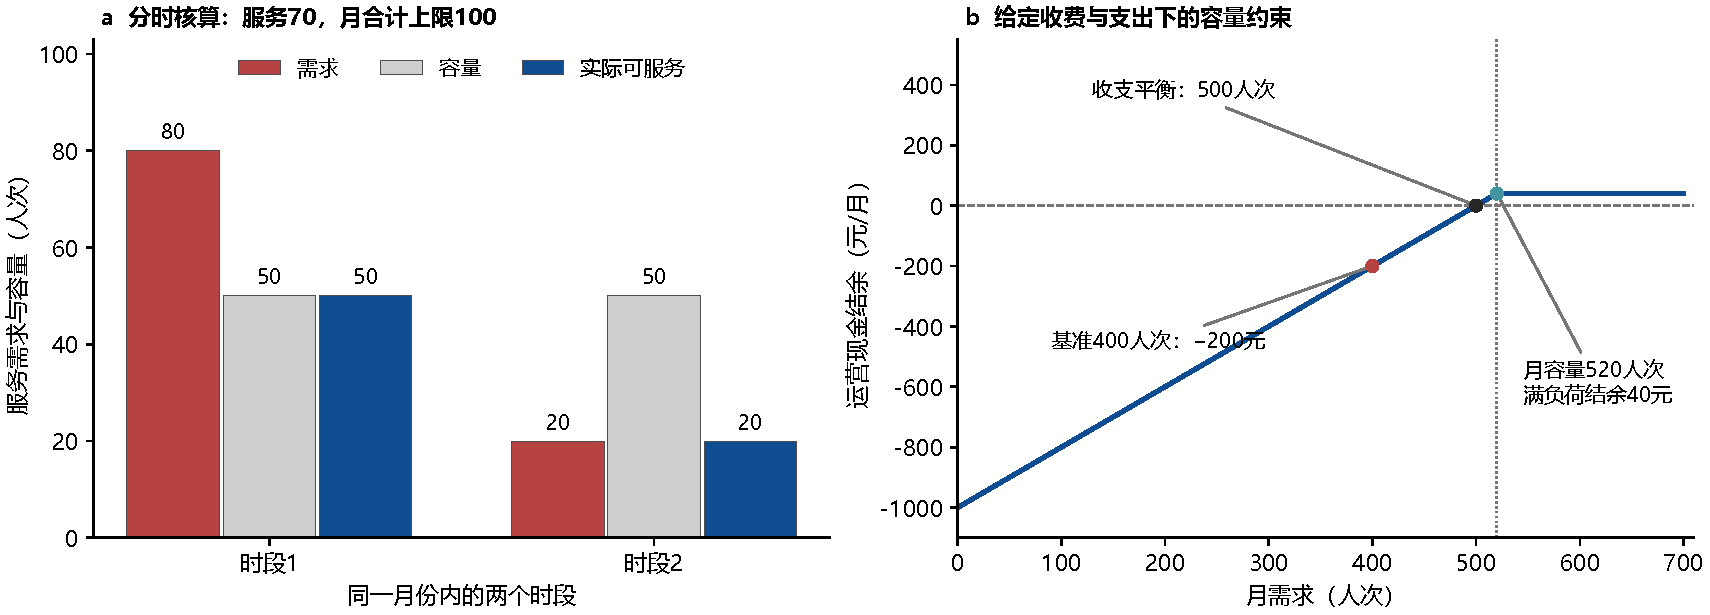
\includegraphics[width=\linewidth]{docs/figures/operations-scientific-checks.pdf}
\caption{同一核算函数的机制检验。a为不可跨时段结转的容量例子；b为给定收费、支出与补贴下的月度需求压力测试。全部为明确标注的演示输入，图中现金边界与表中阈值来自同一结果记录。}
\label{fig:scientific-operations}
\end{figure}

\subsection{把参数范围、单参影响和组合结果一起保存}

系统增加逐参数的下界、基准、上界、范围来源、取得日期及适用说明。单参数分析每次只改一个输入，并调用同一核算函数；组合分析枚举最多6个参数的端点组合。来源不明的百分比不能作为经验分布。\cite{gao2020} 本轮演示以需求倍率0.7至1.3、固定支出9000至11000元测试计算机制，范围性质明确标为人工压力设定。

\begin{center}\small
\begin{tabular}{@{}L{49mm}rrrr@{}}
\toprule 改变的参数 & 下界结余 & 基准结余 & 上界结余 & 结余跨度\\\midrule

固定支出：月度现金事项 & 800 & -200 & -1200 & 2000\\
活动服务：服务需求倍率 & -440 & -200 & 40 & 480\\
\bottomrule\end{tabular}\end{center}
结余及跨度单位均为元/月。四个参数端点组合得到的现金结余为-1440至1040元/月，最大缺口为1440元/月。固定支出的单参跨度为2000元，大于需求变化的480元；在这组演示范围内，固定费用依据更值得优先补充。

这些输出称为“已测试参数组合范围”。若要估计亏损概率或概率覆盖区间，还需有输入分布与依赖关系的依据。JCGM 101要求先依据知识指定输入分布或联合分布，再进行传播计算。\cite{jcgm2008} 本轮不以任意均匀或三角分布把压力测试包装成真实风险概率。

\subsection{两组演示与一个缺项分支}

经济示例采用五年、5\%折现率的演示假设：
\begin{center}\small
\begin{tabular}{lrrl}\toprule
\textbf{模式组合} & \textbf{经营NPV 元} & \textbf{峰值缺口 元} & \textbf{计算状态}\\\midrule
保留整治＋服务运营 & 56,392.31 & 0 & 可开展专项调查\\
部分保留＋局部拆建＋经营 & -285,683.11 & 1,000,000 & 展示调整因素\\
整体拆建，权利与价格缺项 & 空值 & 空值 & 补关键资料\\\bottomrule
\end{tabular}\end{center}

第一方案的保本月租为115.18元/平方米/月。程序保留出资、贷款、收入和业主资产效益的独立账，展示哪些参数使收益或资金缺口变化。这组示例的数据标签均为演示假设。

适老示例采用演示住区1000人、老年占比33\%、目标群体330人；按同一随机序列比较基线与改善，结果如下：
\begin{center}\small
\begin{tabular}{llrrrr}
\hline
组合 & 采用情景 & 可达人数 & 使用人数 & 覆盖率(\%) & 容量使用率(\%) \\
\hline
基线组合 & 低 & 110 & 45 & 13.64 & 28.33 \\
基线组合 & 中 & 110 & 72 & 21.82 & 46.67 \\
基线组合 & 高 & 110 & 91 & 27.58 & 62.22 \\
改善组合 & 低 & 330 & 143 & 43.33 & 53.1 \\
改善组合 & 中 & 330 & 213 & 64.55 & 81.67 \\
改善组合 & 高 & 330 & 235 & 71.21 & 94.05 \\
\hline
\end{tabular}
\end{center}

中采用情景下，去重使用人数由72人增加到213人，增加141人；使用人群覆盖率提高42.73个百分点，月访问量由336次增加到1372次。这是给定人口、路线、设施和采用参数后的预测结果，后续用台账和实际使用记录校准。

演示另保留关键权利、价格或容量字段空值，输出\textbf{“先补充关键资料再判断”}，并显示影响的指标和补填任务。默认缺省的非核心字段只影响其对应规则，其他有完整输入的事项继续运行。

\subsection{用冻结预测和独立对象核验，而非用演示自证准确}

当前应用可冻结预测输入、计算版本、证据和时间，再登记同一中心完整月份的原始台账，保存实际减预测的误差和绝对误差。实际值为0时不计算百分比误差。目标月开始前冻结才归入前瞻对照；事后重建只作历史回放。

后续跨社区检验按社区分组，同一社区的居民记录不能随机拆入训练与测试两侧；跨期检验以较早月份校准、较晚月份验证。数据清理、参数确定和阈值选择只使用校准部分。\cite{groupcv} 本轮已将真实问卷审计、确定性机制检验和月度实绩接口分别实现，实际运营台账尚待取得。

措施展示也采用明确计数单位：项目、案例/规则性质及措施类别相同的记录形成一个默认折叠的措施组，展开后保留不同楼栋、阶段、来源和原卡。宽泛类别中不同原文名称仍可逐项查看。重复提取同一项目、同一来源版本、完全相同字段的记录时复用原卡，不重置复核状态；不同金额、对象或阶段继续分别保存。由此避免把多个原文片段或重复提取误当作多个独立案例。

\subsection{程序应用与复现入口}

现有项目工作台已接入分时录入、收支切换值、带范围依据的敏感性和组合结果；历史工程库支持按面积口径及价格年筛选、显示同口径参考组和排除原因。报告导出保留来源、固定条件、缺项及计算结果，原冻结版本按原值回读。

技术核验分三层：公式与边界测试检查容量守恒、分母和费用重复；HTTP与界面检查录入、保存、读回与导出；真实决策效果留待实际运营台账和独立项目评测。复现采用同一计算入口，表格和图形读取生成结果，关键源文件如下：
\begin{itemize}
\item 月度计算与科学核验：\path{services/capabilities/community_operations.py}、\path{services/capabilities/operations_science.py}。
\item 演示结果复现：\path{scripts/build-scientific-methods-evidence.py}；造价分组复现：\path{scripts/verify-expanded-cost-library.ts}。
\item 用户表接收：\path{scripts/intake-historical-projects-workbook.py}；公开问卷审计：\path{scripts/audit-hangzhou-survey.py}。
\end{itemize}
